\section{Computing Continuum}
\label{sec:example}

Herein we will discuss the challenges of developing a mobile application that exploits the computing continuum, as well as present a running example that will be used throughout the rest of the paper to exemplify our work.

As previously stated, the continuum enables the convergence of many heterogeneous infrastructures, from cloud-hosted virtual machines down to mobile devices. Given that the two fundamental elements of computation are data and behavior, the first major challenge of developing an application that exploits the computing continuum consists in \emph{deciding where in the continuum the data and the behavior should be deployed}. This decision needs to be informed by the profound heterogeneity that exists between the different infrastructures that constitute the continuum. 

Amongst other things one must take into account important QoS aspects, such as availability and latency, as discussed in Section~\ref{sec:intro}. Let us focus, for example, on a continuum that comprises a cloud-based solution, an edge-based infrastructure, and a mobile device. Data and behavior that are deployed to cloud solutions will benefit from high availability, at the cost of introducing higher latency; while data and behavior deployed to an edge-based infrastructure will benefit from a much lower latency, at the cost of having a lower availability as well. A third possibility would be to deploy the data and the behavior exclusively to the mobile device; however, this could lead to important battery drains (see Section~\ref{sec:evaluation}), not to mention other limitations. Balancing these trade-offs at design time can be difficult. The challenge is, therefore, to allow applications to dynamically, and opportunistically, decide where the data and the behavior should be deployed and executed. 

If we focus on behavior, it is common to distinguish between stateful and stateless computation. The main distinguishing factor between stateful and stateless components is that the latter do not produce side-effects, and that their outputs depend solely on their inputs. If we focus on data, it is common to distinguish between mutable and immutable data. While mutable data can be modified after its creation, the same is not true for immutable data. In components that adopt immutable data, the data is initialized once and for all at deployment time.

As we shall discuss in Section~\ref{sec:proposal}, it is our view that the computing continuum should focus on stateless computation with immutable data. Stateless computation with immutable data is much easier to replicate (and test) across the continuum, since no data synchronization is required and any data needed by the computation can be obtained at deployment time. Nevertheless, stateful computation and mutable data cannot always be excluded entirely from modern applications. For these cases we envision a mixed solution in which traditional cloud-based resources are adopted alongside the continuum. 

Developing applications in the computing continuum also poses other important challenges. For example, when selecting where a certain computation should be achieved we need to take into account important \emph{security} aspects, such as \emph{authorization}, \emph{confidentiality}, and \emph{integrity}. Also, deployment and execution in the continuum will need to be supported by \emph{tools}. Tools for performing \emph{integration tests}, \emph{runtime monitoring and adaptation}, etc. will be needed.

Although all these challenges are interesting, and important research endeavors in themselves, in this paper we focus on establishing the basis upon which the computing continuum can evolve. In particular, we focus on achieving (i) the dynamic and automatic deployment of computation by part of the infrastructures that constitute the continuum, and (ii) the opportunistic selection of where to execute the computation.

\subsection{A Running Example}
\label{sub:example}

\begin{figure}[tbp]
	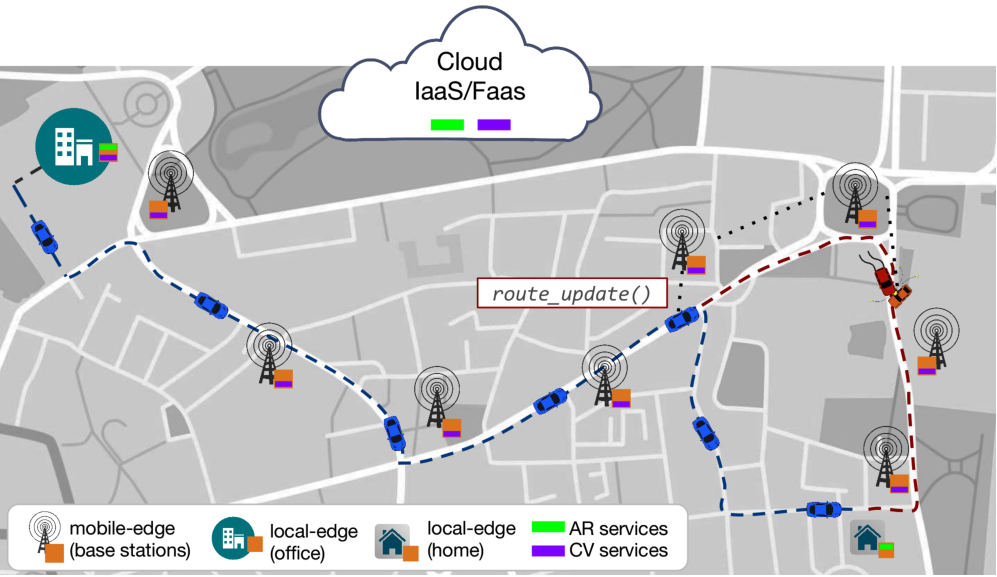
\includegraphics[width=0.9\textwidth]{figs/Continuum-Scenario}
	\caption{Heterogeneous applications such as Augmented Reality (AR), Autonomous Vehicles (AV) and Mobile Games (MG) interact with services deployed along the computing continuum (cloud, mobile-edge, local-edge, and mobile)}
	\label{fig:continuum-scenario}
\end{figure}

%Throughout this section an example scenario (Fig.~\ref{fig:continuum-scenario}) is used to illustrate the use of A3-E model and the cloud-edge-mobile continuum with different applications employed by a person with visual impairment.
We shall now introduce the running example that will be used throughout the rest of the paper to exemplify our work. Figure~\ref{fig:continuum-scenario} shows a complete example scenario that starts in a user's office and finishes at her home. It involves different applications that rely on computation executed in the cloud, edge, or in the user's own devices. 

First, let us assume the existence of a local edge server in the user's office (hereafter called \textit{local-edge}). This server is owned by the company, and it is used to extend the computational capabilities of the devices operated by its employees. In our example, the user makes use of an augmented reality (AR) application to craft virtual 3D objects that are added to her desk table. This application involves heavyweight image processing for the \textit{extraction of features} from the captured scenes, as well as a trained neural network model to \textit{detect objects} from a set of features. With the offloading of both tasks to the local-edge, the user can avoid recharging her glasses and can improve her productivity. Also, the additional storage on the edge servers allows a larger set of objects to be recognized, thanks to a more completely trained model.

After work, the user leaves her offices and enters her autonomous vehicle (AV). During her way home, the vehicle makes use of services deployed at edge servers located at cellular base stations (hereafter called \textit{mobile-edge}) to receive low-latency updates about the best plan to reach her destination. This way, within milliseconds the vehicle can be suggested to adjust its routes to avoid heavy traffic. In particular, let's say that a new path consists of residential streets without mobile-edge coverage. The AV continues to fetch updates, which are now served by a cloud provider. The additional network latency is compensated with the low speed limit of the residential area.

Finally, at home the user can start using her domestic local-edge server. She finds out about a new Mobile Game (MG) application. Upon installation, the local-edge server becomes aware of a new continuum-compliant application and, while the app continues to run locally on her device, it proceeds to setup the services needed to allow the application to offload some of the computation. Once the setup is complete, the application autonomously starts using the edge services with the purpose of preserving the device's resources. Not only does the game's performance improve, battery consumption is also reduced.  

This scenario exploits different parts of the continuum. Traditional cloud resources are employed as a reliable alternative to edge-based computation. Similarly, local services are employed as alternatives to edge services until they have been acquired and made available by a local-edge server. Whilst the transition between mobile-edge and cloud is transparent, the use of local-edge services involves mutual client-server awareness.

